\chapter{Analysis chain}
%

\section{Image Cleaning on the PhotonStream}
%
As pointed out in \autoref{ch:iact} the Cherenkov-light of air-showers shows a
very specific topology. The emitted photons are coherent in space and time:
they originate from a single very high energetic and therefore very fast
primary particle and thus appear in a very brief time window of a few
nanoseconds. Furthermore, the characteristic Cherenkov-angle under which the
light is emitted, creates a light cone, which, when projected to the
$x$-$y$-plane of the camera causes the specific elliptical shape. Both of these
topological features are mandated by the physical process and can therefore be
unrestrictedly used for the cleaning. Background events like ambient light or
starlight don't show these characteristics and tend to appear randomly.

The threedimensional $xyt$-representation of the PhotonStream's point-cloud
quantifies photons with exactly those three observables. Thus, a cleaning
within the threedimensional space-time can heavily use the known topology.
Within the point-cloud, an air-shower will appear as a very dense cluster of
photons, surrounded by a merely isotropic distribution of background photons.
These characteristics of shower events in the PhotonStream representation
naturally suggest a density-based clustering algorithm as the cleaning method
of choice. The two challenges at hand are the choice of a suited algorithm and
a well defined metric to make the threedimensional spacetime usable.

\subsection{Air-showers in the point-cloud}
%
The threedimensional spacetime of the PhotonStream and its representation as a
point-cloud eventually mixes spatial dimensions with time. While this is
physically motivated, defining distances in such a space is not trivial. They
are highly dependant on the chosen metric, which defines how time correspondsto
space. This already implies that the choice of metric contains certain
assumptions and can be adapted to specific preferences. The essential parameter
is the factor $\alpha$, which transfers time to space and vice versa:
%
\begin{equation}
  c_{t} = \alpha \cdot t \, .
  \label{eq:metric}
\end{equation}
%
The choice of this parameter e.g. gives the possibility to prefer spatial
distance over timing information, or the opposite. The spacetime of the
point-cloud is quantized in all its three dimensions: the pixels of the camera
define the spatial grid, whereas the time slices, each event is binned to, do so
for the timing information. When trying to separate air-showers from
background via the density of the shower's photons, the distance plays the
essential role. The natural way to equalize between space and time is to adapt
to the photon distribution of a typical air-shower along each axis. So, by
chosing
%
\begin{equation}
  \alpha = 0.35\cdot10^9\,\si{\degree\per\second}
\end{equation}
%
the one-dimensional density distribution of photons along the coordinates
$c_x$, $c_y$ and $c_t$ is the same. With this metric, the distance between two
photons $a$ and $b$ is defined as
%
\begin{equation}
  d_{a,b} = \sqrt{(c_x^a - c_x^b)^2 + (c_y^a - c_y^b)^2 + (c_t^a - c_t^b)^2}
\end{equation}

The twodimensional projections of the point-cloud within this metric are shown
in \autoref{fig:pc} for an example air-shower event. With the calculated
degree-equivalent of time the air-shower shows a similar distribution in
each dimension.
%
\begin{figure}[H]
  \centering
  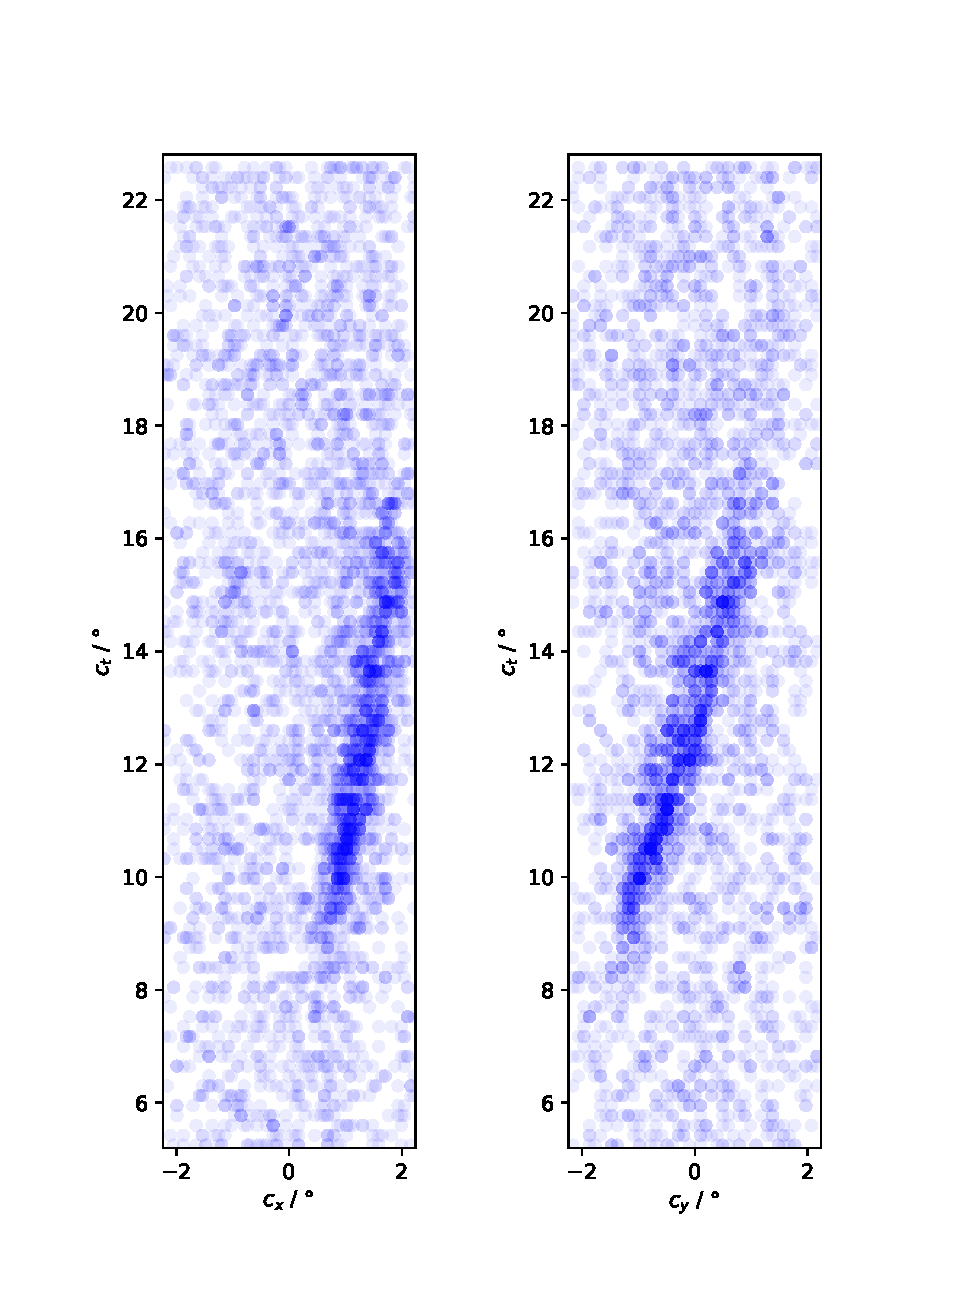
\includegraphics[width=0.6\textwidth, angle=-90]{Plots/point_cloud.pdf}
  \caption{Twodimensional projections of the point-cloud using the metric described above.}
  \label{fig:pc}
\end{figure}
%

\subsection{Density-based Clustering with DBSCAN}
%
To find clusters of photons within the space described above, the PhotonStream
uses the \textit{density-based algorithm for discovering clusters with noise}
(DBSCAN) \cite{DBSCAN}. The DBSCAN is well suited for finding air-showers with the
PhotonStream's observables, when choosing the right parameter set for the algorithm. This
algorithm either assigns each extracted photon to one of potentially multiple
clusters or identifies it as a night-sky-background photon. There are no
assumptions on the shape, location or number of the clusters. The algorithm is
characterized by only two parameters.
%
\begin{description}[align=right]
  \item[m] the minimum number of photons to make up a cluster
  \item[$\symbf{\varepsilon}$] the maximum distance between two photons to be considered dense
\end{description}
%
These two parameters represent the specific topology of the air-shower events
by giving limits on typical shower sizes and spreads in spacetime. For
air-shower events recorded by FACT the best choice was found to be $m = 20$ and
$\varepsilon = \SI{0.45}{\degree}$. So, to survive the cleaning, every found
cluster must at least contain 20 photons within a maximum distance of
$\SI{0.45}{\degree}$ to the respective closest photon. The algorithm determines
the clusters by iterating over the photons in 4 steps:
%
\begin{enumerate}
  \item loop over photons until a dense region with at least $m$ photons is found
  \item add photons to the newly found cluster that are within distance $\varepsilon$ or connected via a chain of dense photons
  \item if nothing to add to cluster restart 1. with leftover photons
  \item mark all photons not assigned to any dense cluster as night-sky-background
\end{enumerate}
%
This way every photon is either belonging to a cluster of an air-shower, or
discarded as background. This determination is taking place in the whole space
of observables the whole time. There are no intermediate steps, only taking
single observables into account, which very much represents a way to find
air-showers in a space well suited for describing them. Furthermore, this way
single photons are selected rather than specific pixels. When expecting
background photons also within signal pixels, this should yield a cleaned image,
closer to the true air-shower image.
%
\begin{figure}
  \begin{subfigure}{0.5\textwidth}
    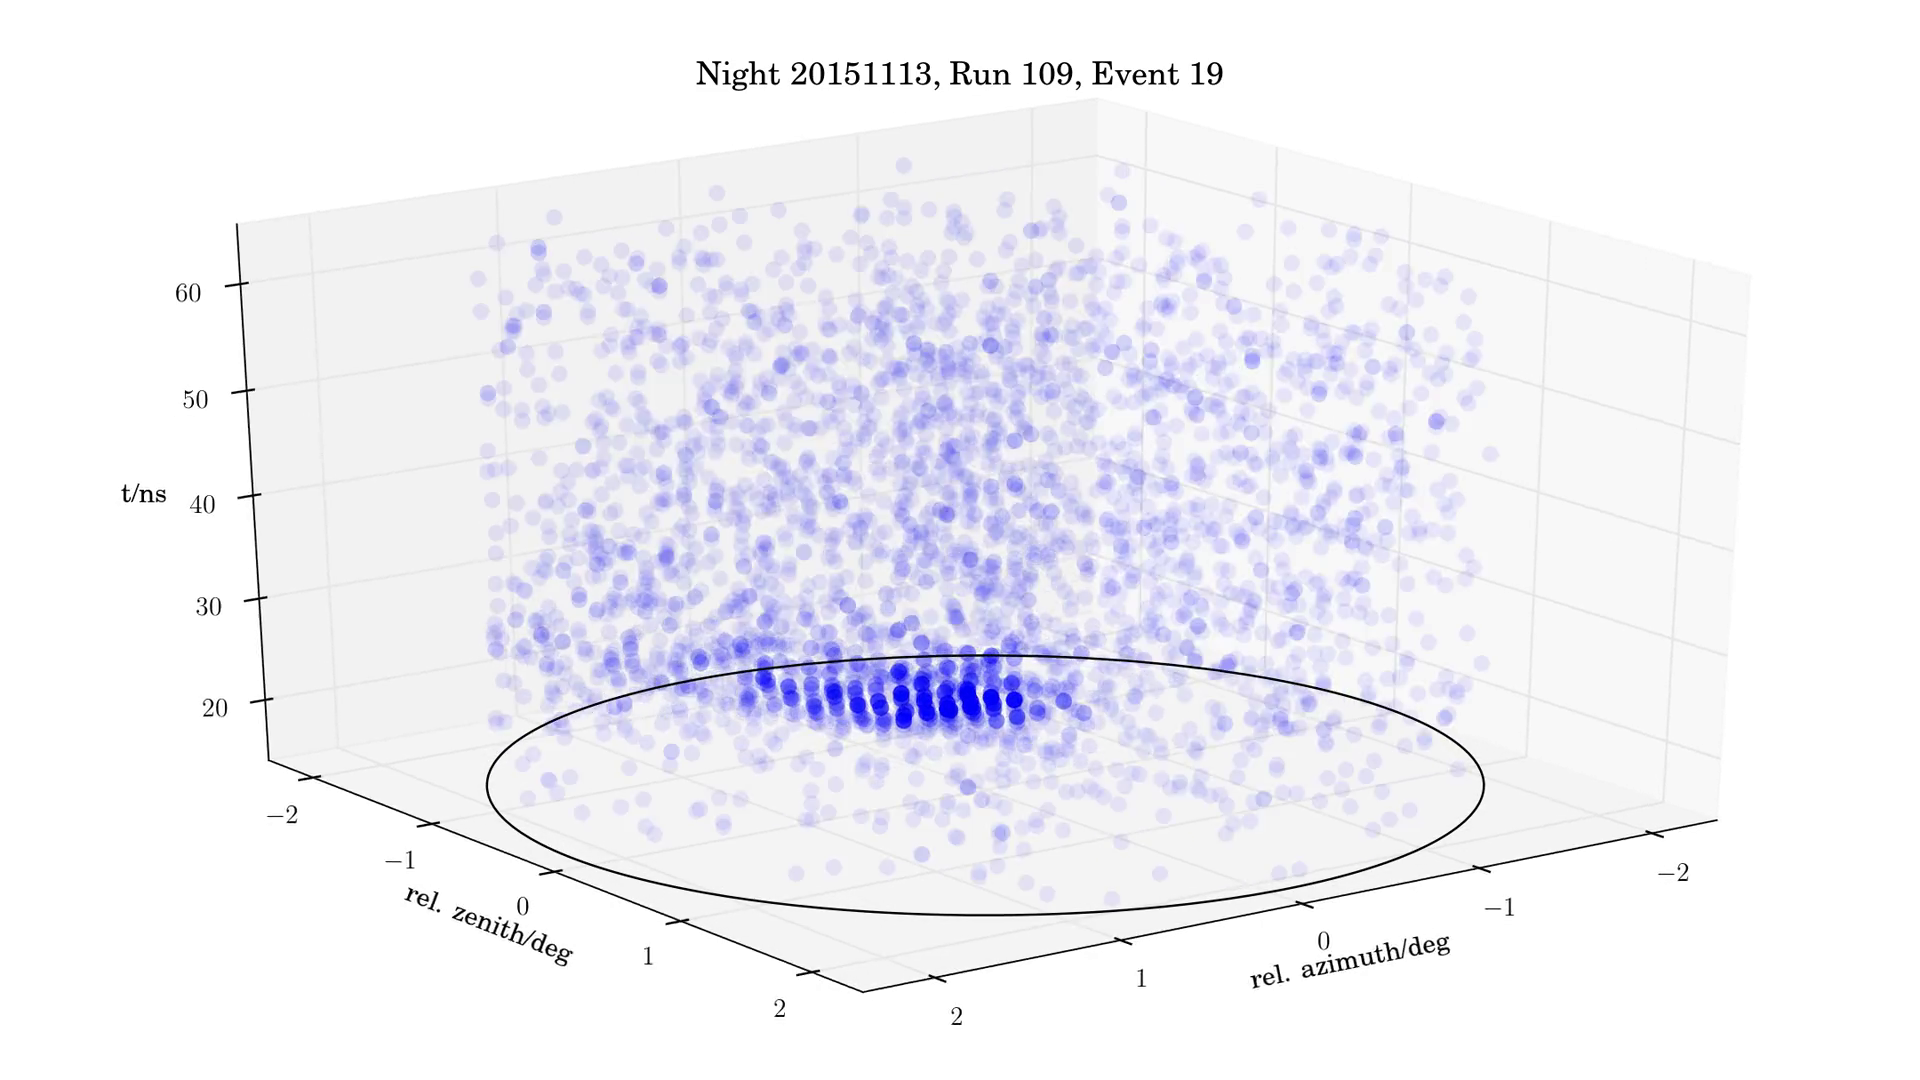
\includegraphics[width=1.1\textwidth]{Plots/event2.png}
  \end{subfigure}
  \begin{subfigure}{0.5\textwidth}
    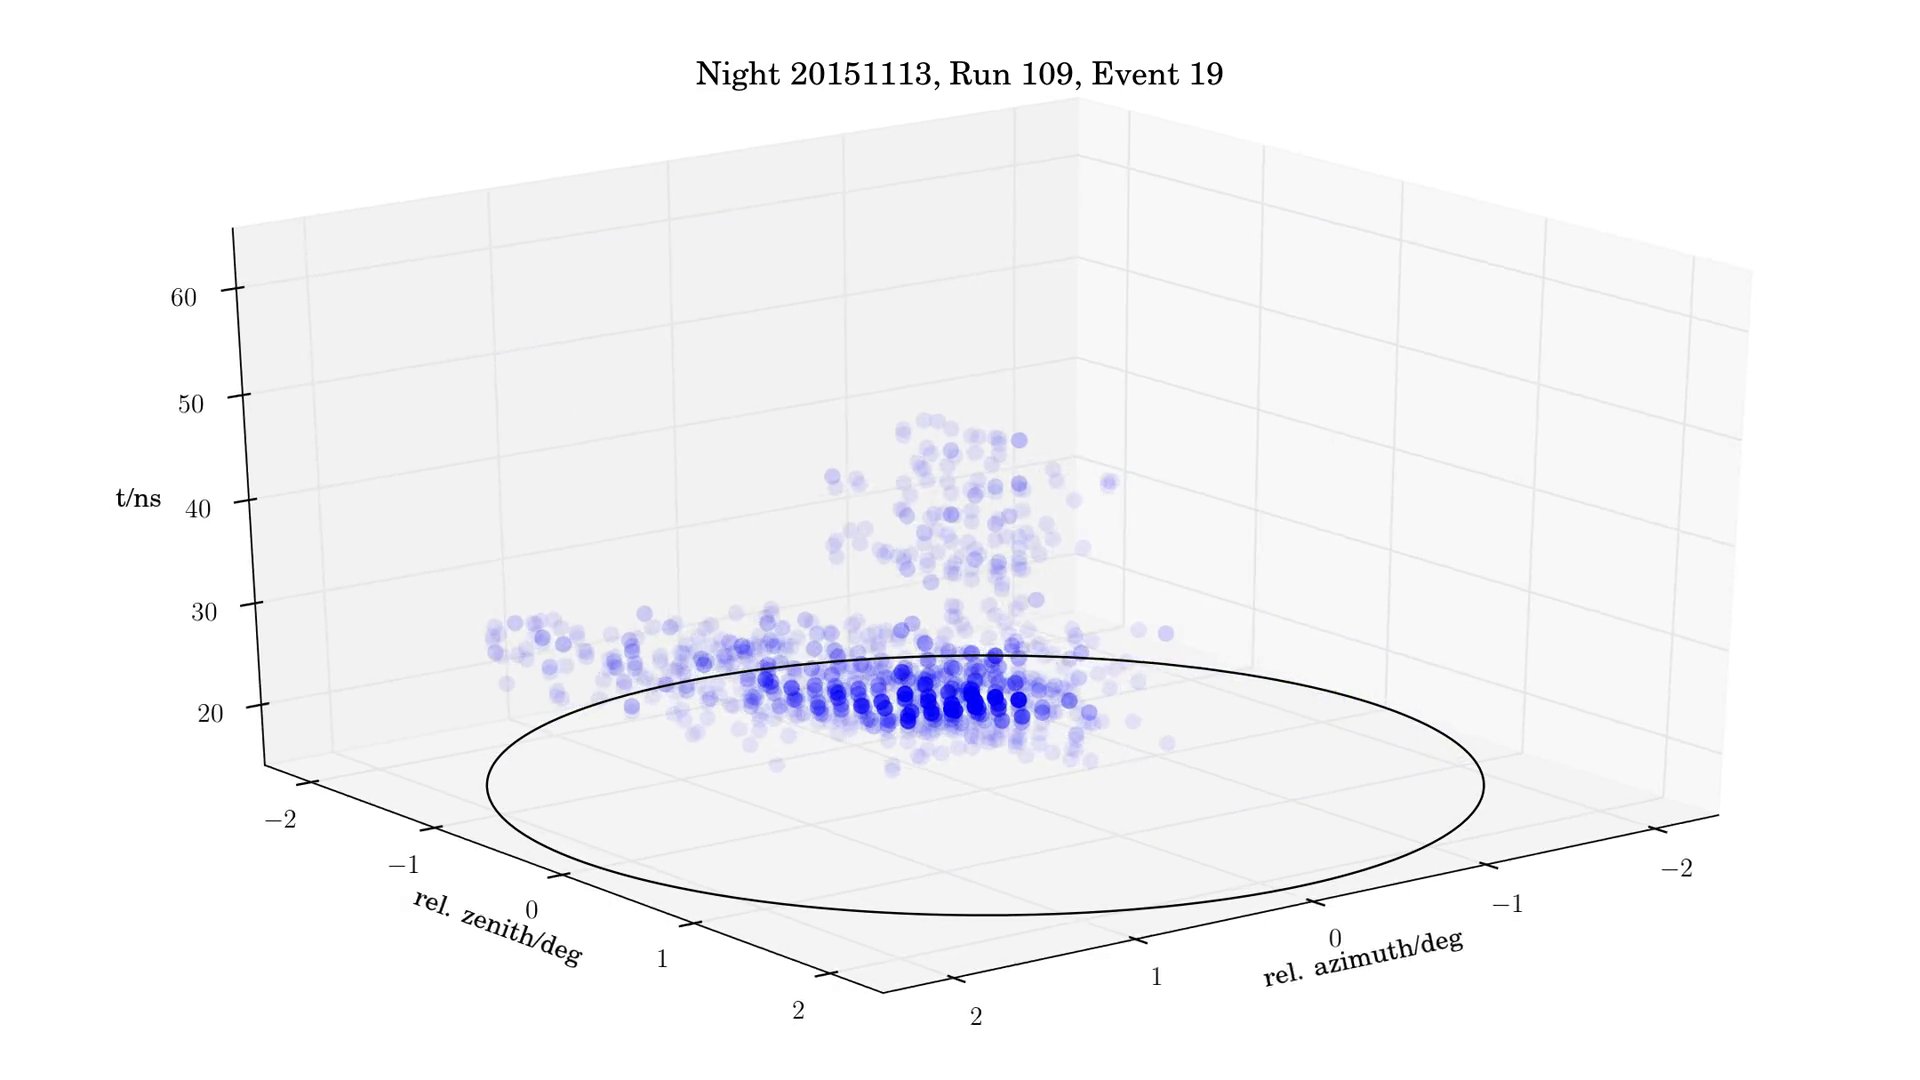
\includegraphics[width=1.1\textwidth]{Plots/event1.png}
  \end{subfigure}
  \caption{Event represented by the 3-dimensional point cloud of the Photonstream. Every blue sphere represents a measured photon in the corresponding time slice and pixel. The right figure shows the remaining photons after cleaning.}
  \label{fig:event}
\end{figure}
%

\section{Parametrization of Events}
%
\begin{figure}
  \centering
  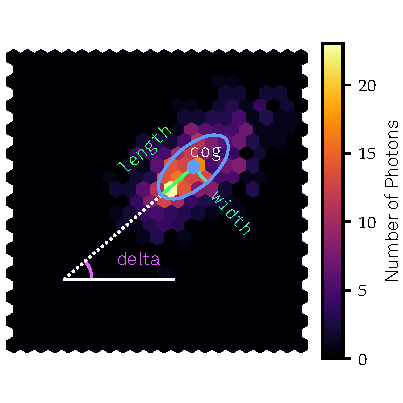
\includegraphics[width=0.6\textwidth]{Plots/hillas2.pdf}
  \caption{Hillas features.}
  \label{fig:hillas2}
\end{figure}
%
%
\begin{figure}
  \centering
  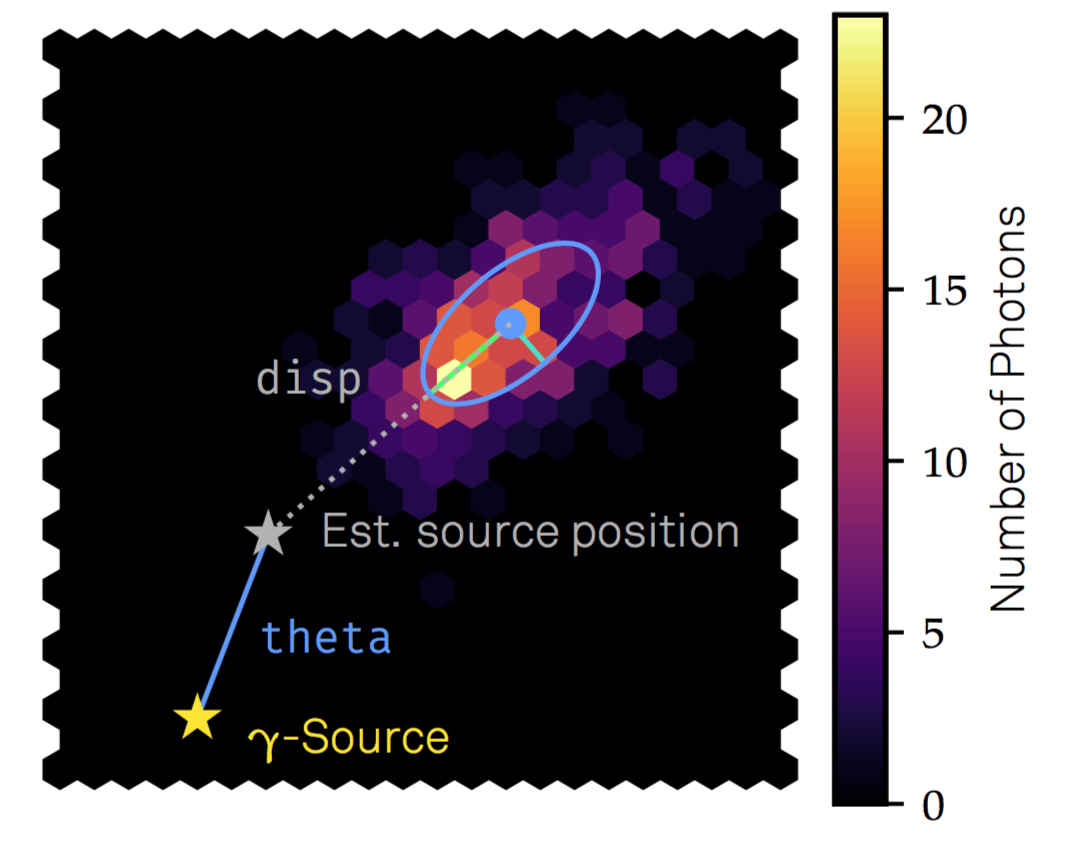
\includegraphics[width=0.6\textwidth]{Plots/disp.png}
  \caption{Disp method.}
  \label{fig:disp}
\end{figure}
%
\section{Image Cleaning with pixelbased Thresholds}
%
\section{Energy Estimation}
%
\section{Reconstruction of the Source Position}
%
\section{Signal-Background Separation}
